\documentclass[11pt]{article}
\usepackage{geometry}                
\geometry{letterpaper}                   

\usepackage{graphicx}
\usepackage{amssymb}
\usepackage{epstopdf}
\usepackage{natbib}
\usepackage{amssymb, amsmath}
\DeclareGraphicsRule{.tif}{png}{.png}{`convert #1 `dirname #1`/`basename #1 .tif`.png}

\usepackage[nottoc,numbib]{tocbibind}

%\title{Title}
%\author{}
%\date{date} 

\begin{document}



\thispagestyle{empty}

\begin{center}

\includegraphics[width=5cm]{ETHlogo.eps}

\bigskip


\bigskip


\bigskip


\LARGE{ 	Complex Social Systems:\\ }
\LARGE{ Modelling Agents, Learning, and Games\\}

\bigskip

\bigskip

\small{Project Report}\\

\bigskip

\bigskip

\bigskip

\bigskip




\centering{
\textbf{\LARGE{A Barcelona Paradox}}\\
Suboptimal Traffic Efficiency in Changing Habitats \\
(SOTECH)
\\
}

\bigskip

\bigskip

\bigskip

\begin{tabular}{@{}c@{}}
\LARGE{Javier Argota Sánchez-Vaquerizo} \\
\normalsize javier.argota@gess.ethz.ch
\end{tabular}%
\quad and\quad
\begin{tabular}{@{}c@{}}
\LARGE{Daniel Schwarzenbach} \\
\normalsize dschwarze@student.ethz.ch
\end{tabular}



\bigskip

\bigskip

\bigskip

\bigskip

\bigskip

\bigskip

\bigskip

\bigskip

Zurich\\
December 2020\\

\end{center}



\newpage

%%%%%%%%%%%%%%%%%%%%%%%%%%%%%%%%%%%%%%%%%%%%%%%%%

\newpage
\section*{Agreement for free-download}
\bigskip


\bigskip


\large We hereby agree to make our source code for this project freely available for download from the web pages of the SOMS chair. Furthermore, we assure that all source code is written by ourselves and is not violating any copyright restrictions.

\begin{center}

\bigskip


\bigskip


\begin{tabular}{@{}p{3.3cm}@{}p{6cm}@{}@{}p{6cm}@{}}
\begin{minipage}{3cm}

\end{minipage}
&
\begin{minipage}{6cm}
\large Javier \\ Argota Sánchez-Vaquerizo

\end{minipage}
&
\begin{minipage}{6cm}

\large Daniel \\ Schwarzenbach

\end{minipage}
\end{tabular}


\end{center}
\newpage

%%%%%%%%%%%%%%%%%%%%%%%%%%%%%%%%%%%%%%%



% IMPORTANT
% you MUST include the ETH declaration of originality here; it is available for download on the course website or at http://www.ethz.ch/faculty/exams/plagiarism/index_EN; it can be printed as pdf and should be filled out in handwriting


%%%%%%%%%% Table of content %%%%%%%%%%%%%%%%%

\tableofcontents

\newpage

%%%%%%%%%%%%%%%%%%%%%%%%%%%%%%%%%%%%%%%



\section{Abstract}

Following the evolution of last urban trends in re-purposing the public space for improving quality of life in cities, there is an increasing shrinkage of space for cars. Among these initiatives, Barcelona Superblocks is one of the most paradigmatic. As frequent in urban planning, the systematic analysis and evidence construction of these interventions are frequently ignored. In this experiment we proposed to analyze the traffic outcomes of the implementation of this Superblocks plan in an idealized Barcelona grid together with other potential scenarios to be as well implemented. By connecting urban interventions in city street networks with their expected outcomes we highlight the promising capabilities of the use of these methods based on modeling and simulation to question, criticise, iterate, and test city making processes in an accessible way for any stakeholder, both experts and lay people.    

\section{Individual contributions}

\begin{itemize}
    \item Javier Argota Sánchez-Vaquerizo was in charge of the data collection and model design and implementation.
    \item Daniel Schwarzenbach reviewed existing Braess Paradox literature and prepared the presentation.
\end{itemize}

\section{Introduction and Motivations}

\subsection {Towards a systematic understanding of urban spaces}

Utilitarian traffic optimization goals has dominated transport engineering since it appears as a proper discipline with the rise of private motorized vehicles. It has shaped our industrial and post-industrial cities that we inhabit. Modern Urbanism, as we understand it nowadays, sinks its roots at into a revolutionary scientific and technical approach towards the understanding of urban environment conditions and the efficient distribution of people, good, and resources around the city \citep{Cerda1867}. Even Modernist urban planners and architects in the early 1900's endorsed a radical mechanistic understanding of cities \citep{CIAM1933}. However, this scientific and positivist approach of traffic engineers contradicts the common practice in urban and city planning. Spatial planning, urban design, and collateral disciplines in the same realm, are affected by a combination of experimental data, domain expertise, ideology, and policy and political constraints in a non-straightforward decision making process in which opposed agendas promoted by different stakeholders are leverage to reach ideally a feasible compromise. In the best case scenario, many urban interventions are based on some domain expertise-backed intuition with the hope of eventually getting people's approval and political adoption.

The understanding of complex effects of spatial planning decisions in cities is still very limited and scarcely applied to common practice. In this context, the assessment of urban interventions in cities frequently lacks evidence support. It undermines any possibility of evaluation of results, iterative process of potential improvement, and proper informed-decision making for technical experts, decision makers, and citizens in general. The later is particularly relevant as this lack of comprehensive information on the effects of planning decisions in cities dismisses the quality of participatory processes, by masking accessible knowledge to people, and making easier to manipulate these processes \citep{Blundell-Jones2005} \citep{Plaza2020}.

\subsection {Barcelona's Superblocks}

This knowledge and methodological gap does not hinder experimentation and innovation in the most complex human creation \citep{Levi-Strauss1955} as cities are. In recent years, there is a clear trend on reducing the space reserved for private motor vehicles in cities to improve air quality and environmental conditions, to foster alternative transportation modes, or to reduce the use of fossil fuels (***citations would be good here*** and as well ***examples of these interventions***). Among these current trends on urban planning, Barcelona's Superblocks has been one of the most published in the last years (***some refs from The Guardian, NYT, etc***). The Superblock's plan aims to reduce the space for the motor private vehicles in the street network to improve living conditions of city inhabitants by reducing noise and air-pollution and giving room to other transportation modes. \citep{Rueda2018} It is being accomplished by creating large blocks of 3-by-3 of current square city blocks and leaving inside only loop-like residential streets. It means that 1 out of 3 streets of the city are left for driving through traffic. The well-known and a-thousands-of-times depicted idiosyncrasy of the so regular Barcelona grid comes together with a long tradition on public engagement on urban planning and experimentation in the city set an ideal scenario for testing out the unknown effect of these and other modifications in urban networks.

\begin{figure}[h]
\centering
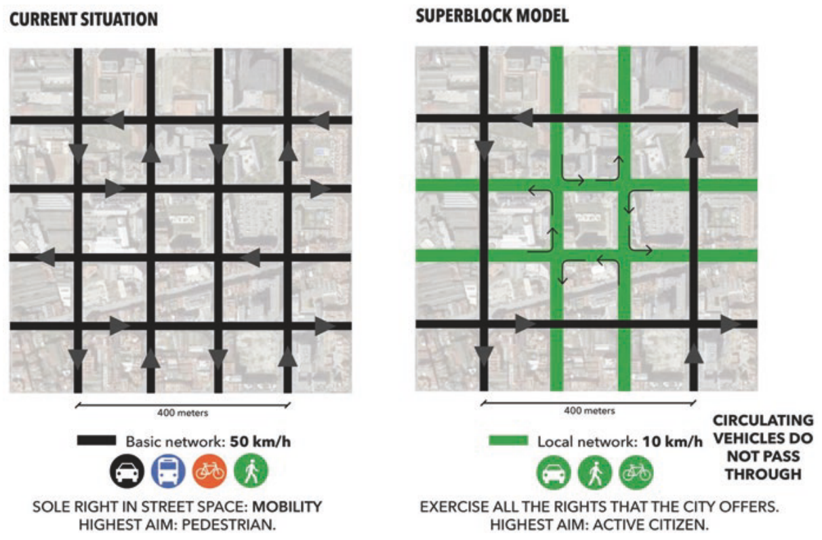
\includegraphics[scale=0.5]{bcn_superblocks_rueda_2018.png}
\caption{Barcelona Superblocks schema \citep{Rueda2018}}
\label{fig:Barcelona Superblocks schema}
\end{figure}

\subsection {The Braess Paradox}

Among one of the most interesting and intriguing effects that defies the common understanding for operating in the urban infrastructures is the so-called Braess Paradox. It explains the counter-intuitive observation that adding more links to a given network, such as a transportation one, can slow down overall traffic flow. It is caused by the selfishly behavior of the entities that are moving in the network when trying to optimize individually their travel time (or cost). It causes to get away from the system optimum. that contrary to the real behavior, requires some level of collaboration between the agents \citep{Braess1969}.

\subsection {Research questions}

\begin{itemize}
    \item Are there too many streets for cars that actually are causing bigger congestion?
    \item If adding new roadways links leads to increased congestion, according to Braess, may removing streets for vehicles cause improvement of traffic, as expected by the Superblocks plan?
    \item Can we apply the counter-intuitive Braess’ Paradox effects for our own benefit in the planning of cities?
\end{itemize}

\subsection {Research Methods}

For modeling and simulating an urban environment to test these changes a microscopic agent-based simulation approach is followed. With this in mind, a common framework applied to transportation modeling in cities called SUMO. This software can simulate virtually any element moving around a city or region as individual agents according to different rules \citep{Lopez2018}.

Additionally, this framework allows to run mesoscopic simulations based on a queueing: it is, instead of simulating every agent behavior independently as in an agent-based approach, every street segment is modeled as a queue of vehicles \citep{Eissfeldt2004}. This approach implies important performance improvements that can be used for simulating larger environments (i.e. an entire city). Consequently, for validating the results of the microsimulation a mesoscopic model is calibrated. It will be as well useful for being able to run larger scenarios more efficiently. 

\section{Description of the Model}

In order to build a simulation in SUMO, two basic elements are needed as initial inputs:
\begin{itemize}
    \item A \textbf{network}, as the representation of the 'physical' environment where agents will move.
    \item  A \textbf{demand} able to generate the movement between the different locations of the environment.
\end{itemize}

\subsection {Network}

The idea behind the used environment is to generalize and abstract the main features defining the regular urban grid of the Barcelona Eixample district. Any particular area of the city of Barcelona is modeled \textit{per se}, but just a representation of the most important features of the urban fabric. This is facilitated by the clear and straightforward ideas that back the Cerda's plan.

An section of the city made of 9x9 Barcelona's blocks is used as the base environment. It is equivalent roughly to 1.44 km\textsuperscript{2}. Each squared block (or if preferred, the distance between the center of the streets intersections) is 133.33 m long. All the streets have the same width and importance (i.e. there is no hierarchy in the urban fabric) and they are one-way, two-lanes, with opposing directions from one block to the following one. Additionally each intersection is regulated with traffic lights whose whole cycle last 90 seconds.

This basic network with the aforementioned parameters represents an idealization or abstraction of the current functioning of the street network in Barcelona (net 1). It is used as the basis for the modified scenarios where different changes are introduced as follows.

Two different settings for superblocks are represented: one made of 2x2 superblocks, and another one with 3x3 superblocks. Both models have been implemented already as pilot project in recent urban refurbishments in the city of Barcelona, although the latter is the original proposed design. Both settings follow the same design principles: major streets separating superblocks are the only ones suitable for cross-city traffic, and their intersections are regulated by traffic lights. Inner streets within each superblock are transformed in residential streets suitable for just residential traffic and other types of transportation. More importantly, for the model design, they are designed as one-lane and one-way loops that do not allow to cross the superblock, which makes impossible cross-city traffic. Consequently, they result into nets 2 and 3.

Finally, a fourth network is included to account for a remarkable feature of the Barcelona grid: the number of diagonal streets that cut the orthogonal grid. For this purpose, the Diagonal Avenue is taken as a reference for capturing its main features to be added to the basic grid. As a result, a diagonal broad street with two-ways and two lanes per direction is added at and angle of 30°. This is net 4.

\begin{figure}[htbp]
\centering
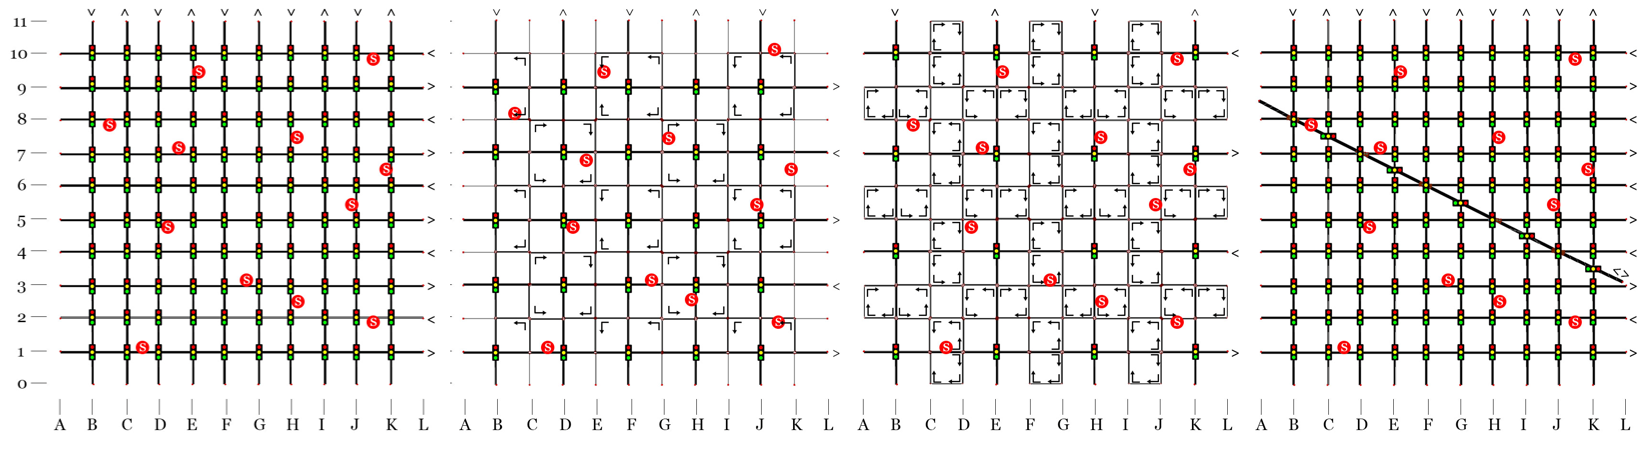
\includegraphics[scale=0.27]{bcn_paradox_4nets.PNG}
\caption{From left to right: Net 1 (basic network), net 2 (2x2 superblocks), net 3 (3x3 superblocks), and net 4 (with diagonal broad avenue).}
\label{fig:From left to right: Net 1 (basic network), net 2 (2x2 superblocks), net 3 (3x3 superblocks), and net 4 (with diagonal broad avenue).}
\end{figure}

\begin{table}[htbp]
\caption{Main metrics for each network.}
\resizebox{\textwidth}{!}{%
\begin{tabular}{p{7em}|p{7em}|p{7em}|p{7em}|p{8em}}

Network & \textbf{Net 1} & \textbf{Net 2} & \textbf{Net 3} & \textbf{Net 4} \\
Description & Basic network & 2x2 superblocks & 3x3 superblocks & w/ diagonal avenue \\\hline
Length of lanes (m)  &               53920&	36588&	34261&	58919 \\ \hline
Length of lanes (\%)  &               100 &	68 & 64&	109 \\ \hline
Number of intersections  &               100 &	25 & 16 &	105 \\ 
\end{tabular}%
}
\end{table}

\subsection {Demand}

For the creation of the demand, two different kinds of mobility need to be considered:
\begin{itemize}
    \item People whose origin and/or destination is within the represented area (i.e. people living and/or working within the network). This *endogenous* demand can be created using the ACTIVITYGEN tool included in SUMO from general demographic data \citep{Lopez2018}.
    \item People exclusively crossing the modeled area (i.e. people who are moving around the city, whose destination is somewhere else out of the represented part of the city). This passing through traffic can be modeled from AADT available data.
\end{itemize}

In general, the regular grid of the city of Barcelona encompasses core urban districts and more residential, suburbial, and even industrial areas whose traffic demands vary largely. In this case, for the considered area, we are assuming that it belongs to a central part of the city which implied higher density of population, of economic activity, of jobs position, and in general of traffic levels (because of inner demand, and passing by population).

Very similarly to the network creation process, we generalize the transportation demand for an equivalent area of the city to the modeled 1.44 km\textsuperscript{2} urban square without representing any concrete neighborhood of the city of Barcelona.

In the case of the transport demand created by *activitygen*, it needs basic demographic data which is extrapolated and generalized for the modeled network area (1.44 km\textsuperscript{2}) based on the Eixample district in Barcelona (7.46 km\textsuperscript{2}) \citep{AjuntamentdeBarcelona2018}\citep{AreadeBarcelona.AutoritatdelTransportMetropolita2020}\citep{DepartamentdAnalisiOficinaMunicipaldeDades.AjuntamentdeBarcelona2020}. This area matches approximately the assumption of the expected mobility intensity for a central part of Barcelona. As a result, the following population statistics are assumed for the modeled area:

\begin{itemize}
    \item 51.120 inhabitant in the area (355 hab/ha x 144 ha)
    \item 2,4 persons per household
    \item Population under 16 yo: 14%
    \item Population 16 - 64 yo: 65%
    \item Population over 64 yo: 21%
    \item Schools (for the whole district): 58 (including primary, middle and high schools, private and public ones). 
    \item Total students 3-16 yo: 24000. Around 70\% stays in the same district, and 30\% move in between districts or municipalities. For the scope of this simulated area, 4800 students are considered (20\%).
    \item Vehicles per 1000 inhabitants: 298.
    \item Share of private vehicle in Barcelona: 22.8\%
\end{itemize}

For generalizing the driving-through traffic three neighborhoods belonging to the Eixample district are chosen as a reference for their inbound and outbound mobility patterns (i.e. people who leave or enter the area in a daily basis) \citep{BestiarioProyectosS.L.2014}. They are the ones showing a more more complex and demanding dynamics: La Dreta de l'Eixample, l'Antiga Esquerra de l'Eixample, and la Nova Esquerra de l'Eixample.

\begin{table}[htbp]
\caption{Demographic and mobility data for reference neighborhood.}
\resizebox{\textwidth}{!}{%
\begin{tabular}{p{10em}|p{10em}|p{10em}|p{10em}}

Neighborhood & \textbf{Dreta de l'Eixample} & \textbf{L'Antiga Esquerra de l'Eixample} & \textbf{La Nova Esquerra de l'Eixample} \\ \hline
Total population                 & 43449 & 42189 & 57889 \\ \hline
Area (km2)                       & 2.12  & 1.23  & 1.34  \\ \hline
Density (hab/km2)                & 20500 & 34355 & 43200 \\ \hline
Outbound mobility (\% tot. pop.) & 30    & 32    & 32    \\ \hline
Inbound mobility (\% tot. pop.)  & 138   & 66    & 32    \\ 
\end{tabular}%
}
\end{table}

Averaging these mobility patterns, we can assume for the model:
\begin{itemize}
    \item Outbound mobility: 31.4\% of tot. population of the model
    \item Inbound mobility: 74\% of tot. population of the model
\end{itemize}

Finally, these total daily values can be adjusted to an hourly distribution of trips during the day for generating random trips (see randomTrips.py script from SUMO) between the fringe edges (i.e. streets situated on the limit of the network that are used for entering and exiting the model). In this case the hourly distribution of the trips is obtained from the histogram generated by the ACTIVITYGEN tool used for the endogenous demand. 

As a result, a total of 315000 vehicles are included into the model by adding the vehicles from the endogenous demand and the driving through traffic.

The initial validation of this demand modeling is performed immediately by comparing the outcomes of the hourly histogram of modeled trips to the measured total trips by the metropolitan authorities in Barcelona \citep{AreadeBarcelona.AutoritatdelTransportMetropolita2020} and the expected counting of vehicles in a similar area from the real AADT \citep{AjuntamentdeBarcelona2016}.

\section{Implementation}

The proposed experiments assumed that the demand does not change in each of the fours networks designed. What changes is the topological and spatial features of the urban fabric, not the transportation demand which remains the same.

In order to perform a sensitivity analysis and increase the scenarios considered, a scaling factor is applied to the demand. Starting from a scale factor of 1 equals to the basic demand modeling extracted from the real data (i.e. 315000 vehicles), the same simulation is run 40 times, spanning from a scale of 0.05 (equivalent to a low demand case of only 15750 vehicles) up to a scale of 2.0 (which equals 630000 vehicles, the double of the current basic scenario), in increments of 0.05 (it is, adding 15750 vehicles). This approach allows to explore a large range of traffic demands and identify the different behavior that the proposed network can face. 

\section{Simulation Results and Discussion}

\section{Summary and Outlook}

\bibliographystyle{plain}
\bibliography{references}





\end{document}  



 
